\clearpage{\pagestyle{empty}\cleardoublepage}
\chapter{Background e Contesto}                %crea il capitolo
%%%%%%%%%%%%%%%%%%%%%%%%%%%%%%%%%%%%%%%%%imposta l'intestazione di pagina
\lhead[\fancyplain{}{\bfseries\thepage}]{\fancyplain{}{\bfseries\rightmark}}
\pagenumbering{arabic}                  %mette i numeri arabi

In questo primo capitolo verrà discussa la problematica dell'inquinamento atmosferico.
Saranno elencate le sue cause ed i suoi effetti, e si discuterà sulle modalità tramite le quali viene diffusa la consapevolezza sull'argomento.
Questo capitolo introduttivo si occuperà di fornire il contesto in cui si inserisce il progetto di tesi, prestando particolarmente attenzione all'utilizzo di varie metodologie di rappresentazione dei dati; soffermandosi, in particolare, sui pregi e difetti di queste, proponendo inoltre delle alternative non del tutto convenzionali.

\section{L'inquinamento dell'aria}
Con inquinamento atmosferico, si intendono tutte le alterazioni alla normale composizione chimica, fisica e biologica dell’atmosfera; o più semplicemente dell’aria che respiriamo.
Possiamo dividere le principali cause del peggioramento dell’aria in due categorie: naturali e antropiche.
\\
Le cause naturali dell'inquinamento riguardano principalmente eventi climatici ed ambientali, come ad esempio le eruzioni vulcaniche e le piogge acide.
Questi fenomeni esistono dapprima dell'uomo e non possono essere evitati, nonostante questo; gli inquinanti naturali non rappresentano una minaccia particolarmente seria per la salute umana.
\\
L'inquinamento antropico è invece dovuto alle azioni dell'uomo. Le principali cause di questo sono l’uso di combustibili fossili come il carbone, il petrolio e il gas naturale.
In seguito alla combustione, queste risorse rilasciano sostanze nocive, come ad esempio il monossido di carbonio, la CO\textsubscript{2} e i metalli pesanti.
Fortunatamente, le politiche di tutela dell'ambiente sono sempre più attente a questo problema;
non sono poche neanche le campagne di sesnibilizzazione il cui fine è quello di istruire la popolazione sull'argomento. Questi eventi sono organizzati da enti riconosciuti a livello internazionale e nazionale, come ad esempio l'associazione ambientalista Legambiente: l'associazione dei cittadini per la difesa dell'ambiente ~\cite{la_mincrometrologia}.
\\
\subsubsection{Relazione tra inquinamento e territorio}
Possiamo definire l'inquinamento antropico come una causa della civilizzazione e dell'industrializzazione: il peggioramento della qualità dell'aria è infatti strettamente legato all'urbanizzazione, caratterizzata dall'aumento della popolazione e dei loro bisogni di trasporto, di energia e di beni di consumo.
La relazione tra uomo e inquinamento è molto complessa ed osservabile sotto vari aspetti di cause ed effetto.
Il modo in cui la popolazione si distribuisce nel globo ha un forte impatto sull'ambiente.
Già nel 1999, circa metà della popolazione mondiale (47\%) viveva in aree urbane, a causa della migrazione verso le grandi città ~\cite{population_and_enviroment}.
Questo ha portato, specialmente nelle regioni meno sviluppate, ad un inevitabile surclassamento dell'urbanizzazione rispetto allo svilupo di tecnologie sostenibili e di politiche di tutela dell'ambiente ~\cite{population_and_enviroment}.
\\
Altri fattori che influenzano il preggioramento dell'aria non sono direttamente legati alla popolazione, ma alle caratteristiche naturali del territorio.
La presenza di polveri sottili nell'atmosfera è uno degli aspetti cruciali che influenzano la qualità dell'aria.
Seppure presenti anche in natura, nelle rocce e nelle sabbie, le polveri sottili più nocive sono di causa antropica, e si concentrano nelle metropoli.
Un fenomeno da non sottovalutare è quello del rimescolamento: le particelle inquinanti possono essere trasportate da un luogo all'altro seguendo le correnti di vento, mescolandosi con l'aria pulita.
Il rimescolamento non è però sempre un fenomeno negativo, in quanto può “omogeneizzare”, e quindi mitigare, il livello di inquinamento in un'area molto vasta, riducendo la concentrazione di inquinanti in possibili centri abitati ~\cite{la_mincrometrologia}.

\subsection{Riferimenti legislativi}
In Italia, il principale decreto legislativo che tratta la tematica di inquinamento dell'aria è il 155/2010 “Attenuazione della direttiva 2008/50/UE relativa alla qualità dell'aria ambiente e per un'aria pulita in Europa”.
Le normative emanate in questo decreto si pongono come obbiettivo quello di ridurre l'inquinamento atmosferico, attraverso l'adozione di misure di prevenzione e di controllo.
Il provvedimento individua per ogni Regione gli enti al quale delegare l'utilizzo di strumenti utili alla misuara dell'inquinamento e l'attuazione di piani di prevenzione e risanazione dell'aria.
Il punto principale del decreto è quello di stabilire quali sono le sostanze inquinanti e quali sono i loro livelli massimi tollerabili (Figura \ref{fig:livelli}), al fine di tutelare la salute umana, in particolare quella dei soggetti più deboli ~\cite{arpa_veneto}.
\begin{figure}
  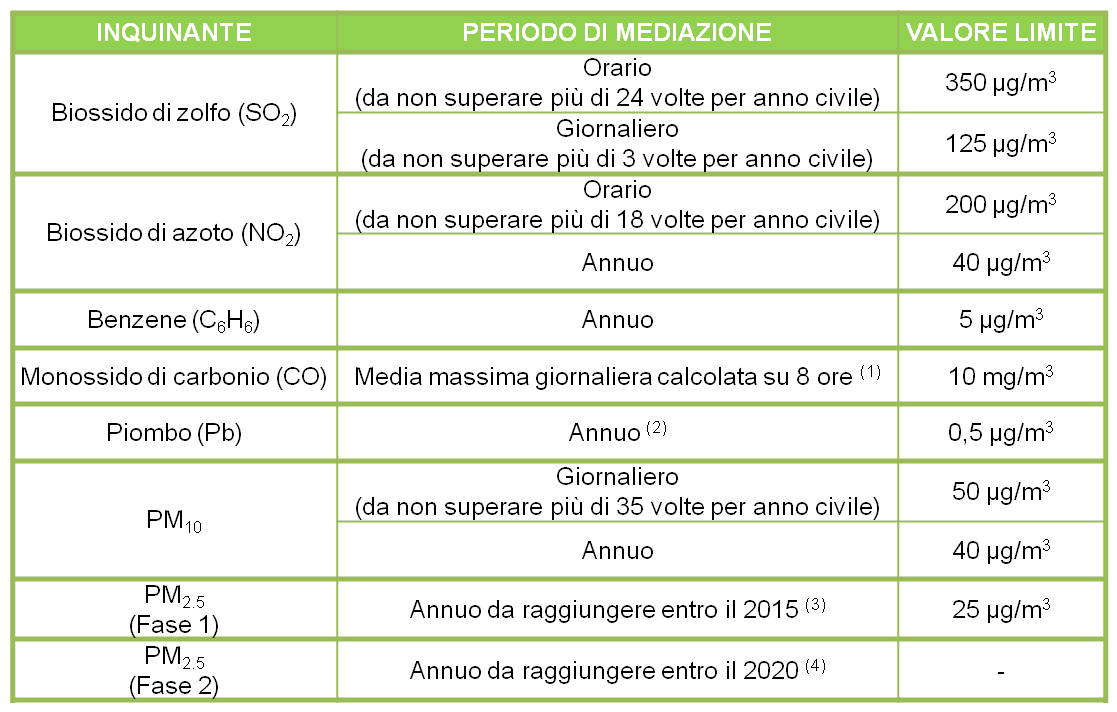
\includegraphics[width=\linewidth]{img/livelli.png}
  \caption{Concentrazione massima tollerata per agente inquinante secondo il decreto 155/2010 ~\cite{aqitable}.}
  \label{fig:livelli}
\end{figure}


\subsection{Misurare l'inquinamento}
Per conoscere il livello di qualità dell’aria in una determinata località, è necessario rilevare la concentrazione di ogni elemento nocivo. 
L'ente principale che si occupa di monitorare l'inquinamento atmosferico è la WHO: World Health organization.
\\
La misurazione effettiva dell'inquinamento è delegata alle amministrazioni locali, che si occupano di installare i sensori necessari per rilevare la concentrazione di ogni sostanza.
Negli Stati Uniti, L'EPA è il leader sulla ricerca e sullo sviluppo di strumenti e tecnologie per misurare l'inquinamento atmosferico.
Nell'Unione Europea, invece, questo compito è affidato all' EEA: European Environment Agency.
\\
Ciascuna di queste oraganizzazioni si occupa inoltre di effettuare piani di prevenzione e precauzione per ridurre l'inquinamento all'origine, rivolgendosi alle imprese più impattanti sull'ambiente con la formula “polluter pays”, che vuol dire che chi inquina paga ~\cite{polluter_pays}.
\\ 
Per semplificare la rappresentazione della condizione dell’aria, l’EPA ha introdotto l’AQI (air quality index): una misurazione semplice e generalizzata.
Ulteriori indici che verranno discussi in questa tesi sono il PM2.5 e il PM10, le cui metodologie di rilevazione sono standardizzate e normate dalla WHO.
Questi valori sono calcolati in base alla concentrazione di particolato aereodisperso di grandezza inferiore a 2.5 e 10 micrometri per metro cubo, rispettivamente.
L'accumulo di queste polveri sottili nell'aria è ciò che viene comunemente definito come smog.
\\
Le particelle sottili PM2.5 sono particolarmente dannose per la salute umana, in quanto possono penetrare con molta semplicità nell'organismo, fino ad arrivare ai polmoni e ai globuli rossi.
Alcuni effetti a lungo termine dell'esposizione a queste sostanze sono la diminuzione della capacità respiratoria, l'infiammazione dei polmoni e la riduzione della capacità di difesa del sistema immunitario ~\cite{pmrisk}.
\subsubsection{Approfondimento sull'AQI}
L'AQI è un indice che misura la qualità dell'aria in un'area geografica.
La sua formulazione è la seguente: ad una determinata zona viene associato un valore numerico, compreso tra 0 e 500, più questo valore è alto, più l'esposizione all'aria rappresenta un rischio per la salute ~\cite{aqibasics}.
In generale, le zone con un valore aqi inferiore al cento sono considerate “buone”, seppure non perfettamente sane, mentre quelle con un aqi superiore a questo valore non rispecchiano gli standard di sicurezza.
La semplicità di questo indice ne caratterizza la sua efficacia, l'AQI è ormai diventato uno standard internazionale per valutare la qualità dell'aria.
L'indice AQI viene calcolato a partire da 5 dei principali agenti inquinanti:
\begin{itemize}
  \item{la concentrazione di polveri sottili (pm2.5 e pm10);}
  \item{il livello di ozono ad altezza della crosta terrestre;}
  \item{il livello di diossido di zolfo;}
  \item{il livello di diossido di nitrogeno;}
  \item{il livello di monossido di carbonio.}  
\end{itemize}
Infine, per ottenere una singola misurazione AQI si calcola la media di più misurazioni avvenute in un arco di tempo, solitamente di 1 ora, 8 ore e una giornata intera ~\cite{aqibasics}.
	
\definecolor{Green}{rgb}{0.0,0.8,0.0}
\definecolor{Yellow}{rgb}{1.0,1.0,0.0}
\definecolor{Orange}{rgb}{1.0,0.5,0.0}
\definecolor{Red}{rgb}{1.0,0.0,0.0}
\definecolor{Purple}{rgb}{0.6,0.0,0.8}
\definecolor{Maroon}{rgb}{0.6,0.6,0.6}

\begin{table}[h]
  \centering
  \caption{Qualità dell'aria in base all'indice AQI ~\cite{aqibasics}.}
  \label{tab:aqi}
  \begin{tabular}{|c|c|c|}
    \hline
    AQI & Qualità dell'aria & Rischi per la salute \\ \hline
    \rowcolor{Green} 0-50 & Ottimale & Nessun rischio \\ \hline
    \rowcolor{Yellow} 51-100 & Accettabile & Lievi rischi per i soggetti deboli \\ \hline
    \rowcolor{Orange} 101-150 & Non buona & Maggiori rischi per i soggetti deboli \\ \hline
    \rowcolor{Red} 151-200 & Cattiva & Possibili rischi per tutta la popolazione \\ \hline
    \rowcolor{Purple} 201-300 & Molto cattiva & Seri rischi per tutta la popolazione \\ \hline
    \rowcolor{Maroon} 301-500 & Pericolosa & Nessuno dovrebbe uscire \\ \hline
  \end{tabular}
\end{table}

%%%2%%%
\section{Visualizzazione dei dati}
Per ridurre l'inquinamento atmosferico, è necessario conoscere la sua distribuzione e la sua intensità.
La sola disposizione di dati non è però sufficiente per rendere la situazione comprensibile a tutti.
La soluzione più semplice per diffondere consapevolezza è fornire una rappresentazione grafica delle informazioni sull'argomnto.
\subsection{La data visualization}
Con data visualization si intende il processo di rappresentazione di dati numerici o testuali tramite grafici, immagini, animazioni o qualsiasi altro formto grafico ~\cite{data_visualization}.
La data visualization è una delle principali tecniche utilizzate per lo studio dei dati: sotto forma visiva, infatti, è possibile eseguire analisi in maniera più rapida e semplice ~\cite{data_visualization}.
\\
La data visualization è un aspetto fondamentale per la comunicazione; il suo utilizzo spazia in tantissimi campi di attività:
dalla statistica con l'utilizzo di grafici, alla divulgazione metereologica, tramite l'utilizzo di mappe ~\cite{data_visualization}.
Rappresentare graficamente un dato, non è mai un processo solamente tecnico, ma anche creativo.
Per essere esaustiva, chiara e comprensibile, una visualizzazione deve essere progettata con cura e attenzione. La prima cosa da tenere in conto è il tipo di dati che si vuole rappresentare; non tutte le varie forme di data visualization sono adatte a tutti i tipi di dati.
Un'aspetto fondamentale da considerare è la scelta dei colori da utilizzare.
I colori hanno un effetto emotivo che diffcilmente le parole sono in grado di esprimere: se associato ad un contesto e a del testo, ogni colore assume infatti un significato diverso.
La sensazione che un utente prova alla visione di un colore dipende fortemente dal suo stato d'animo, dalla personalità e dalla provenienza; ragione per la quale il significato di ogni colore ha radici culturali e antropologiche ~\cite{color_symbolism}.
\\
Prima di arrivare al risultato finale, è necessario svolgere un'ultimo passaggio: il preprocessing dei dati.
Con preprocessing dei dati si intendono tutte le trasformazioni che vengono eseguiti su questi per renderli più adatti alla visualizzazione.
Alcuni esempi di preprocessing includono  la normalizzazione dei dati e la rimozione di dati errati oppure duplicati.

\subsection{Rappresentare l'inquinamento}
Per fornire una rappresentazione grafica dell’inquinamento, è necessario avere a disposizione una serie di dati, questi vengono solitamente messi a disposizione da enti come l'EPA e l'EEA.
\\ 
Solitamente, le formule preferite per una raffigurazione non troppo scientificamente dettagliata dell’inquinamento sono i grafici e le mappe interattive.
I grafici sono utili per spiegare l'andamento di una serie di dati, come ad esempio la concentrazione di un inquinante in un determinato periodo di tempo.
Gli stili di grafico più comuni per questo scopo sono i grafici a barre, per rappresentare dati discreti, e i grafici a linee, per rappresentare le varie rilevazioni di un dato nel tempo.
\\ 
Le mappe interattive vengono utilizzate per spiegare ad un utente la relazione tra un dato e il territorio sul quale questo è stato registrato, mettendo a disposizione funzioni come lo zoom e la ricerca per località.
Le mappe interattive offrono un ottimo contesto e geografico e, arricchite dall'utilizzo dei colori giusti, sono uno strumento efficacissimo per la comunicazione (esempio in Figura \ref{fig:pollution_map}).
La mappa si presta per essere riempita con qualsiasi tipo di dato: possiamo attribuire ad ogni zona un colore differente, disegnare delle linee o dei poligoni, o ancora aggiungere dei marker interattivi.
Utilizzando simultaneamente più metodi di visualizzazione differenti, possiamo comunicare all'utente più informazioni in un'unica schermata, fornendo anche la possibilità di comprendere le relazioni tra questi; queste mappe vengono comunemente chiamate mappe multilayer o multistrato.
\begin{figure}[H]
  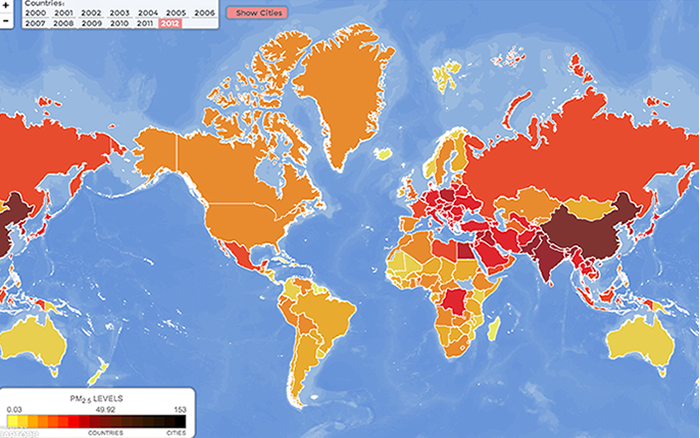
\includegraphics[width=\linewidth]{img/mappapm.png}
  \caption{Una mappa sul livello di particelle pm2.5 ~\cite{aqimap}.}
  \label{fig:pollution_map}
\end{figure}


\subsection{I problemi della rappresentazione grafica}
Nonostante l’auto esplicabilità, il solo utilizzo della data visualization porta con sé diversi svantaggi. 
Il problema principale consiste nella totale assenza di feedback che un grafico offre al lettore.
\\
Prendiamo come esempio un grafico che mostra l'accumulo nel tempo delle polveri sottili nell'aria riempito con dati molto preoccupanti. 
Un utente, la cui preparazione sulla materia viene unicamente dalla legenda del grafico stesso, rischia di attribuire un peso sbagliato a quanto visualizzato ~\cite{disadvantages}.
\\ 
Un ulteriore problema della visualizzazione non animata, risiede nell'impossibilità di fornire all’interlocutore la percezione del tempo. 
Se ogni rilevazione di un grafico corrisponde ad una giornata differente; tramite le sole immagini risulta difficile comprendere quanto tempo richiedono dei processi come la risanazione dell'aria o lo spargimento delle polveri sottili.
\\ 
Infine, se dovessimo spostarci in un contesto ben più complesso dell’inquinamento atmosferico, come ad esempio un grafico astrofisico, è semplice pensare all’aumento della difficoltà nel rappresentare i dati. 
In questi contesti, seppure ancora un'ottima risorsa, la sola data visualization non è sufficiente per rendere delle informazioni comprensibili a non esperti.


%%%3%%%
\section{Sonificazione}
\subsection{Definizione di Sonificazione}
Con sonificazione si intende il processo tramite il quale dei dati di qualsiasi natura vengono trasformati in elementi acustici ~\cite{hermann}.
Più semplicemente, la sonificazione prende dei dati come input, e produce un suono come output. In Figura \ref{fig:sonification_scheme} viene mostrato lo schema riassuntivo del processo di sonificazione.
Il principio sul quale si basa questa tecnica è quello dell'auditory display, ovvero l'uso del suono per rappresentare delle informazioni.
La tecnica dell'auditory display risale a ben prima dell'informazione digitale, il semplice utilizzo di sirene e campane per attirare l'attenzione è solo uno dei possibili esempi.
Con il passare del tempo, questo principio ha trovato sempre più applicazioni nel settore dell'informatica, fino al 1992, anno nel quale è stato fondato l'International Community for Auditory Display (ICAD): il forum di ricerca più importante al mondo in questo campo.
Durante la sedicesima edizione dell'evento, il ricercatore Thomas Hermann, ha definito delle proprietà che ogni sistema di sonificazione deve possedere ~\cite{hermann}:
\begin{itemize}
  \item{il suono deve riflettere le proprietà dei dati rappresentati;}
  \item{la generazione del suono deve essere sistematica, i criteri tramite i quali il suono viene generato devono quindi essere chiari;}
  \item{la sonificazione deve essere deterministica, ovvero il suono prodotto deve essere sempre lo stesso per un dato input;}
  \item{il sistema deve essere riutilizzabile sia con gli stessi dati molteplici volte, sia con dati differenti.}
\end{itemize}
\begin{figure}[H]
  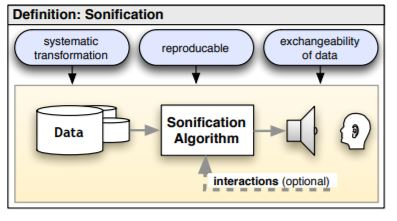
\includegraphics[width=\linewidth,scale=0.5]{img/schema.png}
  \caption{Lo schema riassuntivo della sonificazione ~\cite{hermann}.}
  \label{fig:sonification_scheme}
\end{figure}


\subsection{L'utilizzo della sonificazione}
Il principale utilizzo della sonificazione è quello di fungere da alternativa alla data visualization, oppure arricchirla, tramite lo stimolo di un ulteriore senso: l’udito ~\cite{soni_temporal}.
\\ 
Degli studi svolti sul campo della cinematografia e dell’intrattenimento in generale, sono arrivati alla conclusione che l’audio è la componente chiave per connettere lo spettatore con quello che sta vedendo. 
Uno dei metodi tramite i quali il cervello ritiene molto coinvolgente una rappresentazione grafica arricchita da una traccia audio consiste infatti nell’associazione di pattern visivi ad un certo suono.
In altre parole, il cervello è in grado di comprendere le informazioni uditive più semplicemente di quelle visive; l’orecchio infatti distingue meglio le tonalità di una traccia audio di quanto l’occhio riesca a leggere i vari colori ~\cite{audiovideo}.
\\
Con abbastanza inventiva, tramite la sonificazione è possibile trasformare qualsiasi informazione in suono, in questa tesi, ci concentreremo sui grafici.
Una semplice strategia per la sonificazione di un grafico consiste nell'associare un impulso sonoro tanto sgradevole quanto negativo sia il dato da rappresentare.
Tramite questa tecnica agli utenti risulterà molto più semplice interpretare quanto visualizzato.
\\ 
La sonificazione dei grafici è inoltre un ottimo modo per rappresentare i dati offrendo all’interlocutore una migliore percezione del tempo ~\cite{soni_temporal}. In un grafico nel quale ogni rilevazione è identificata da una giornata differente, 
se associamo ad ogni dato una nota o, più in generale, un suono, all’utente risulterà sicuramente più semplice avere una migliore cognizione soggettiva del tempo trascorso.
\\ 
\subsubsection{Rappresentare dei dati multidimensionali}
Tramite la sonificazione, è semplice rappresentare in maniera chiara dei dati in forma multi dimensionale, come ad esempio, i grafici tridimensionali. 
Per rappresentarene le diverse proprietà di ogni dato nei grafici tridimensionali, è possibile associare a ognuna di queste uno dei vari aspetti dell'audio, come ad esempio il volume e la tonalità ~\cite{multidimensional}.
\subsubsection{La musica generativa}
La sonificazione può essere usata come strumento per la creazione di musica generativa.
Come ogni tipo di arte generativa, la musica generativa si riferisce alla creazione di una canzone in parte o totalmente da un sistema autonomo.
La caratteristica di questa tecnica è che il risultato non può essere ripetuto, in quanto infinito e sempre diverso.
In questo contesto, la sonificazione si presta molto bene per la creazione di musica, in quanto non segue i canoni della musica tradizionale.
Solitamente, una traccia sonificata, non distingue mai un inizio, una fine o un ritornello, ragione per la quale è possibile msuicare un flusso di dati potenzialmente infinito ~\cite{generative_music}.

\subsection{Sonificazione ed accessibilità}
La sonificazione è un ottimo modo per rendere i dati accessibili ad individui portatori di disabilità visiva, come ad esempio, cecità completa o parziale.
Solitamente, le persone con disabilità visiva, per poter comprendere delle informazioni, si affidano a un terzo che legge per loro; spesso sotto forma di un software screen reader.
Questi software incontrano sempre grandi difficoltà nel leggere qualsiasi tipo di immagina, e quindi, anche i grafici.
La sonificazione risolve questo problema, permettendo al persona non vedente di comprendere le informazioni tramite la percezione uditiva, se affiancata ad una descrizione testuale leggibile da un screen reader ~\cite{accessibility}.
\\
La rappresentazione uditiva di è inoltre molto utile per le persone affette da daltonismo.
Alcune forme di data visualization utilizzano unicamente la simbologia dei colori per trasmettere informazioni; un possibile esempio legato al discorso dell'inquinamento consiste in una mappa dove ogni stato stato è colorato in base alla qualità dell'aria.
Affiancare ad ogni paese un determinato suono, oltre che un colore, rende la rappresentazione molto più comprensibile a persone affette da questa disabilità.

\subsection{Adattare un dato ad un formato sonoro}
Per creare una traccia audio coinvolgente, è possibile usare simultaneamente più aspetti dell'audio, i principali sono:
\begin{itemize}
  \item{il volume;}
  \item{la durata;}
  \item{la tonalità: quanto una nota è acuta;}
  \item{il timbro: cio che caratterizza il suono di uno strumento;}
  \item{la stereofonia: tramite l'utilizzo di due canali audio (ad esempio delle cuffie), è possibile creare un effetto di spazio e distanza tra i suoni.}
\end{itemize}
Le modalità di adattamento di un dato ad un formato sonoro sono solitamente stabilite dallo sviluppatore stesso, in base al formato dei dati a disposizione e al tipo di sensazione che si vuole trasmettere.
Vengono utilizzati principalemente tre approcci: l'audificazione tramite sintesi sonora, il design sonoro o sonificazione acustica, e la creazione di modelli di sonificazione ~\cite{soni_temporal}.
Di segutio verranno presentate le tre modalità, evidenziando le loro caratteristiche, le limitazioni, le possibili applicazioni e le loro differenze.
\subsubsection{La sintesi sonora}
Se si vuole solamente fornire una rappresentazione alternativa a quella visiva, un'ottimo approccio per la creazione del suono è la sintesi sonora.
Con sintesi sonora si intendono le tecniche tramite le quali, con l'ausilio di hardware e software, un suono viene generato da zero, senza utilizzare strumentazione acustica ~\cite{izotope}.
Nel processo di sonificazione tramite sintesi, i dati vengono convertiti in una funzione periodica matematica.
Senza entrare troppo nel dettaglio, un possibile esempio di sonificazione tramite sintesi, consiste nell'ottenere l'onda sinusoidale più vicina ai punti in un grafico; le proprietà di quest'onda, quali frequenza e ampiezza, descrivono il suono che verrà prodotto.
\\
Una serie di dati, alternativamente, può essere trasformato in serie di campioni, comunemente chiamati wavetable.
Per suonare diversi toni musicali, vengono riprodotti i campioni audio ad intervalli regolari in base alla frequenza che si vuole ottenere ~\cite{serum}.
Solitamente il numero di campioni utilizzati è 8192, un numero abbastanza alto da rendere riproducibile qualsiasi frequenza udibile dall'orecchio umano. Un esempio di Wavetable è disponibile in Figura \ref{fig:wavetable}.
\begin{figure}[H]
  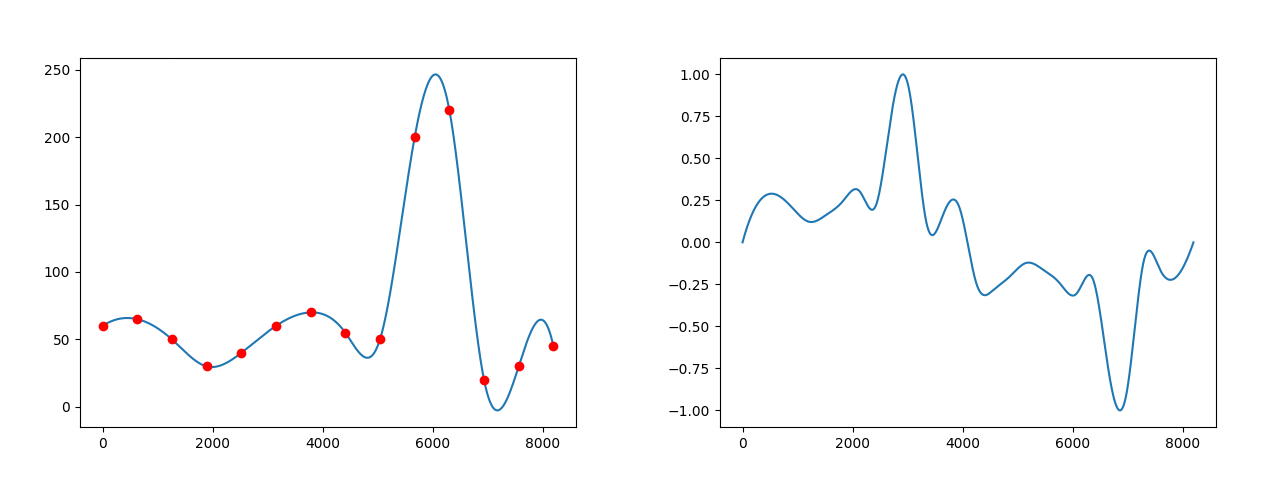
\includegraphics[width=\linewidth]{img/image.png}
  \caption{Una wavetable che ho generato a partire da dei dati sull'inquinamento.
  A sinistra, in rosso, sono raffigurate le rilevazioni dell'inquinamento. L'onda sonora periodica, mostrata a destra, è frutto dell'interpolazione, attenuazione e ripetizione di questi.}
  \label{fig:wavetable}
\end{figure}

 
Per quanto interessante, il suono creato con la sintesi è spesso poco espressivo.
La principale causa di questo fatto è la mancanza di armonici, ovvero le frequenze che si sommano alla frequenza fondamentale (quella che denomina la nota), solitamente responsabili per definire il timbro di uno strumento o di una voce umana.
\subsubsection{Design sonoro}
Un secondo possibile approccio consiste nell'utilizzare suoni di strumenti reali: un semplice esempio potrebbe coinvolgere l'utilizzo di suoni gradevoli e rilassanti per rappresentare dati positivi, e suoni sgradevoli per rappresentare dati negativi.
\\ Nel processo di sonificazione, si possono applicare inoltre nozioni di composizione musicale e design sonoro: l'andamento dei dati può essere infatti rappresentato dalle note di una scala, di un accordo o di qualsiasi altra forma di melodia.
La teoria musicale insegna inoltre a fare provare delle determinate emozioni all'ascoltatore; gli accordi e le scale maggiori esprimono emozioni positive, mentre le tonalità minori esprimono emozioni negative.
Se invece volessimo indurre una sensazione di timore per rappresentare un dato particolarmente negativo, potremmo utilizzare un suono molto forte e acuto, o, più in particolare, una dissonanza.
La dissonanza è un suono che non è in accordo con una scala musicale, risultando quindi fuori contesto e sgradevole ~\cite{dissonance}.
Un designer sonoro può infine aggiungere alla propria traccia sonificata l'utilizzo di filtri e effetti audio digitali.
Tramite questi, è possibile ottenere un suono più ricco e complesso, che rispecchi meglio la natura dei dati.

\subsubsection{Model Based Sonification}
Un ultimo approccio di sonificazione, meno interessante dai due precedenti a livello implementativo, consiste nel creare modelli sonificativi.
Un modello di sonificazione è un sistema in grado di generare una risposta acustica quando un utente vi interagisce.
Per creare un modello, l'ideatore deve per prima cosa associare ad un evento ad una determinata azione, in seguito stabilire le modalità di interazione e infine procedere con la realizzazione.
A differenza della sintesi audio e del design sonoro, un modello è solamente in grado di rispondere a segnali esterni secondo regole predefinite, e non è in grado di generare suoni autonomamente.
Un esempio di modello di sonificazione è il theremin: uno strumento musicale elettronico tramite il quale un musicista, allontanando e avvicinando le mani alle antenne dell'oggetto, modifica la frequenza e l'ampiezza del suono prodotto ~\cite{sonification_model}.


\subsection{Esempi spiegati}
Il primo impiego effettivo della sonificazione risale al 1908. Lo studioso Hans Geiger si pose il problema di dare una rappresentazione immediata e di facile interpretazione della quantità di raggi gamma e particelle beta presenti nell’aria.
Inventò così il contatore Geiger: un dispositivo in grado di fornire un feedback sonoro in tempo reale sul livello di radiazione presente in un’area.
Il principio di sonificazione utilizzato nel contatore Geiger è molto semplice: lo strumento suona dei “click” ad intervalli regolari; più la concentrazione di radioattività è alta più il tempo di attesa tra i vari click si riduce ~\cite{soni_temporal}.
\\\\
Con il passare del tempo, il concetto di sonificazione si è adattato a rappresentare dati di ogni natura, e non solo quelli legati a proprietà fisiche, diventando a tutti gli effetti una alternativa alla visualizzazione grafica.

\subsubsection{Sonificare il prezzo di Bitcoin}
\begin{figure}[H]
  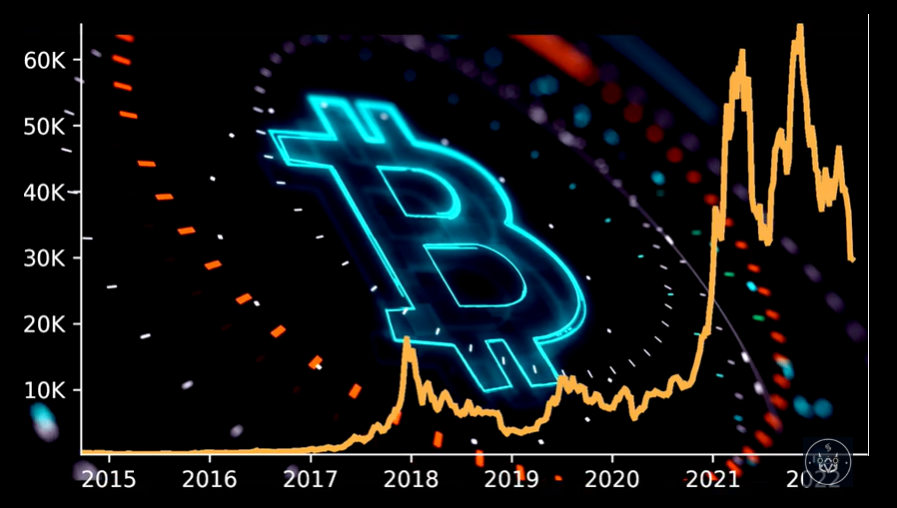
\includegraphics[width=\linewidth]{img/btc.PNG}
  \caption{L'andamento del prezzo del bitcoin tra il 2015 e il 2022, rappresentato con un grafico azionario  ~\cite{bitcoin}.}
  \label{fig:btc}
\end{figure}
Il grafico in Figura \ref{fig:btc}, è stato sonificato dal data scientist Rohith Teja  ~\cite{bitcoin}.
Questo esperimento si differenzia da molti altri per la particolare gradevolezza del suono prodotto, anche ad un orecchio non esperto.
Per raggiungere questo scopo, il lo studioso ha utilizzato la sonificazione solamente per generare la sequenza di note; associando ad ogni variazione di prezzo del bitcoin una nota musicale.
Il suono vero e proprio è prodotto da dei sintetizzatori virtuali anni 80', all'interno di una Digital Audio Workstation: un software professionale per la produzione musicale.
Come base musicale Rohith ha scelto un'armonia di do maggiore, ovvero un set di note che possono essere suonate insieme.
Ogni dato presente nel grafico è mappato su una nota dell'armonia con un criterio molto semplice: più il prezzo del bitcoin è alto, più la nota è acuta.
E' stato utilizzato un insieme di note molto armonioso data la positività dei dati rappresentati.
\\\\


\subsubsection{Trasformare un'immagine in campioni audio}
Vediamo invece un esempio che utilizza la sintesi audio.
\begin{figure}[H]
  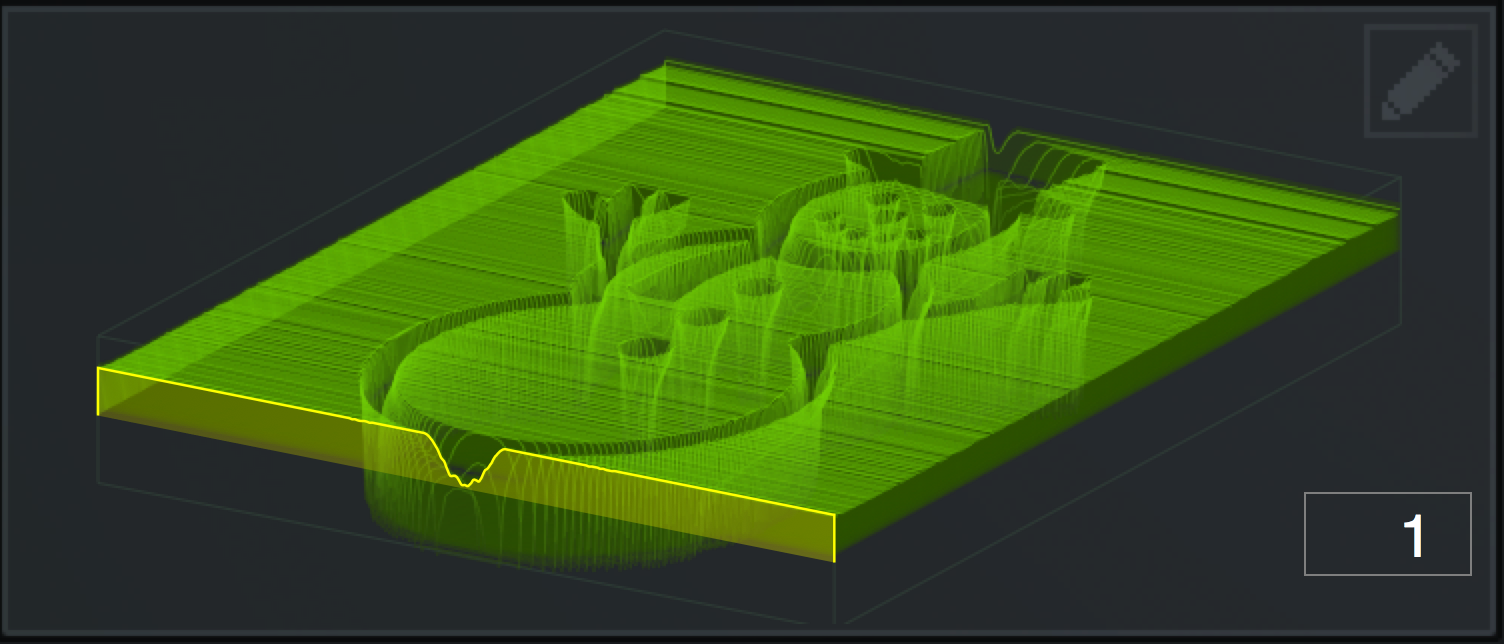
\includegraphics[width=\linewidth]{img/snowman.png}
  \caption{La rappresentazione sonora di un'emoji \cite{snowman}.}
  \label{fig:emoji_wavetable}
\end{figure}

Nell'immagine \ref{fig:emoji_wavetable}, viene mostrata una delle funzioni messe a disposizione dall'Xfer Serum, un sintetizzatore virtuale ~\cite{serum}.
Questa feature permette di sonificare qualsiasi immagine importata nel programma secondo vari criteri.
Il criterio più semplice consiste per prima cosa nel convertire l'immagine in scala di grigi, e di ridimensionarla in un quadrato di dimensioni prefissate.
A partire da ogni riga dell'immagine viene poi generata una sequenza di campioni, ognuno dei quali mappato sul livello di luminosità del singolo pixel.
Tramite questo processo è possibile dare una rappresentazione sonora ad immagini come radiografie, fotografie di satelliti o rilevazioni di sensori.

\subsubsection{Sonificare la volta celeste}
Durante la ricerca, le sonificazioni che più ho apprezzato riguardano la rappresentazione sonora dello spazio.
La cosa in comune tra questi esperimenti è la loro capacità di trasmettere un senso di grandezza e di infinità, accentuato dall'utilizzo del riverbero: l'effetto acustico ottenuto simulando la riflessione del suono in un ambiente. 
Sul sito della NASA, sono disponibili molti esempi di sonificazione di dati astronomici, ognuno dei quali utilizza approcci differenti ~\cite{nasa}.
Analizzando, ad esempio, la galassia NGC 1569, i ricercatori hanno deciso di rappresentare i tre colori principali dell'immagine con tre intervalli di frequenza differenti; in aggiunta, il livello di luminosità determina il volume di ogni suono.
Grazie questa strategia, è possibile distinguere, sia od occhio che a orecchio, i vari corpi celesti presenti nell'immagine.
Questa sonificazione utilizza un approccio bottom-top, consiste ovvero nel trasformare ogni riga dell'immagine in un suono e di concatenare questi in sequenza. 

